% !TeX spellcheck = it_IT
\newpage
\section{Trasformazione di schemi}
L'obiettivo della trasformazione è quello di ottenere da uno schema concettuale uno schema \textbf{logico-relazionale} che rappresenti gli stessi dati in maniera \textbf{corretta} ed \textbf{efficiente}, riducendo la ridondanza e facilitandone la comprensione.\\
Questa trasformazione prende in \textbf{ingresso} lo schema relazionale, il carico applicativo e il modello logico e restituisce in \textbf{uscita} uno schema logico e la documentazione.\\
Si compone dei seguenti passi:
\begin{enumerate}
	\item Rappresentazione delle associazioni uno ad uno e uno a molti
	\item Rappresentazione delle associazioni molti a molti o non binarie
	\item Rappresentazione delle gerarchie di inclusione
	\item Identificazione delle chiavi primarie
	\item Rappresentazione degli attributi multivalore
	\item Appiattimento degli attributi composti
\end{enumerate}

\begin{example}[Esempio di trasformazione]
	Dato il seguente schema concettuale
	\begin{center}
		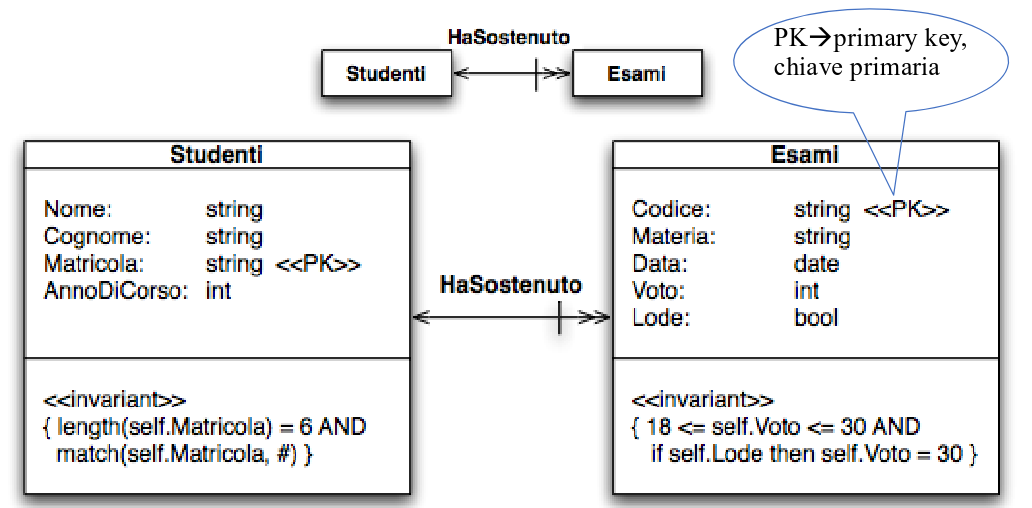
\includegraphics[scale=0.35]{esempiotrasformazione.png}
	\end{center}
	per ottenere uno schema logico introduciamo l'attributo \textbf{matricola}. Questo ci porta ad avere due relazioni collegate dal nuovo attributo.
	\begin{center}
		\begin{tabular}{|c|c|c|c|}
			\hline
			\textbf{Nome} & \textbf{\underline{Matricola}} & \textbf{Provincia} & \textbf{AnnoNascita} \\
			\hline
			Isaia & 071523 & PI & 1982 \\
			\hline
			Rossi & 067459 & LU & 1984 \\
			\hline
			Bianchi & 079856 & LI & 1983 \\
			\hline
			Bonini & 075649 & PI & 1984 \\
			\hline
		\end{tabular}
	\end{center}
	\begin{center}		
		\begin{tabular}{|c|c|c|c|}
			\hline
			\textbf{\underline{Materia}} & \textbf{\underline{Candidato*}} & \textbf{Data} & \textbf{Voto} \\
			\hline
			BD & 071523 & 12/01/06 & 28 \\
			\hline
			BD & 067459 & 15/09/06 & 30\\
			\hline
			FP & 079856 & 25/10/06 & 30 \\
			\hline
			BD & 075649 & 27/06/06 & 25 \\
			\hline
			LMM & 071523 & 10/10/06 & 18 \\
			\hline
		\end{tabular}
	\end{center}
\end{example}
\newpage
\subsection{Rappresentazioni}
\subsubsection{Uno a molti/uno}
\paragraph{Uno a molti}
Le associazioni uno a molti si rappresentano aggiungendo agli attributi della relazione rispetto a cui l’associazione è univoca una \textbf{chiave esterna} che riferisce l’altra relazione. Se l’associazione ha degli attributi, questi si aggiungono alla relazione in cui è presente la chiave esterna.

\begin{center}
	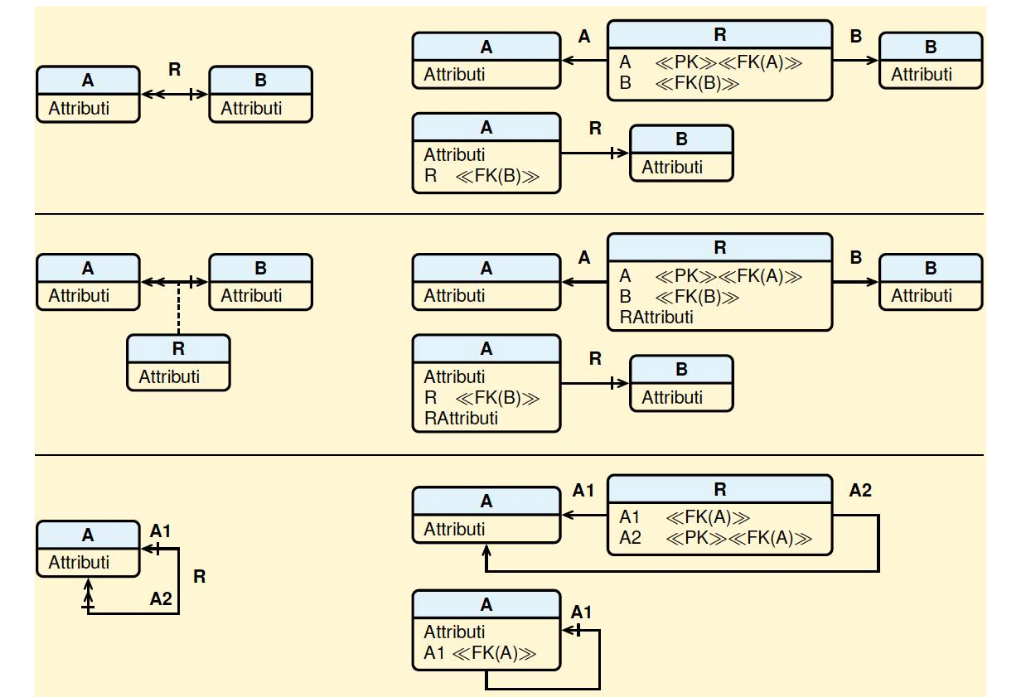
\includegraphics[scale=0.4]{trasfunomolti.png}
\end{center}

\paragraph{Uno ad uno}
Le associazioni uno a uno si rappresentano aggiungendo la \textbf{chiave esterna} ad una qualunque delle due relazioni che riferisce l’altra relazione, preferendo quella rispetto a cui l’associazione è totale, nel caso in cui esista un vincolo di totalità.
\begin{center}
	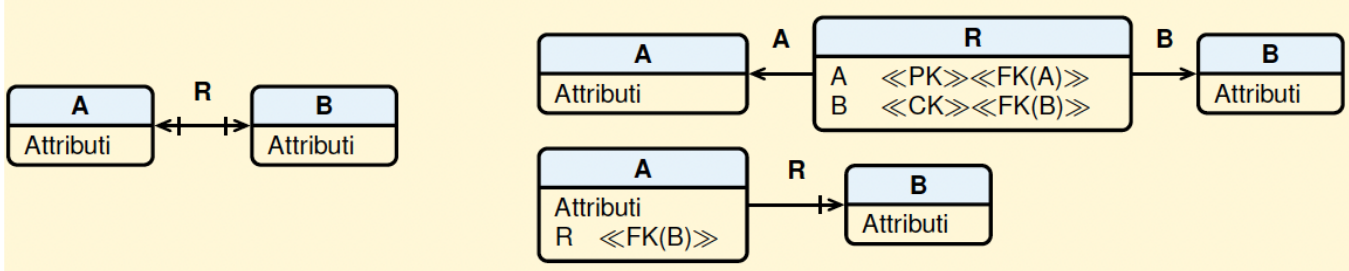
\includegraphics[scale=0.3]{trasfunouno.png}
\end{center}

\paragraph{Vincoli}
\begin{definition}[Diretta]
	La direzione dell’associazione rappresentata dalla chiave esterna è	detta \textbf{la diretta} dell’associazione.
\end{definition}

I vincoli sulla \textbf{cardinalità} delle associazioni \textbf{uno ad uno} e \textbf{uno a molti} sono:
\begin{itemize}
	\item \textbf{Univocità} della diretta
	\item \textbf{Totalità} della diretta: vincolo \textit{not null} sulla chiave esterna
	\item \textbf{Univocità} dell'inversa e \textbf{totalità} della diretta: vincolo \textit{not null} e \textit{di chiave} sulla chiave esterna
\end{itemize}
\subsubsection{Molti a molti}
Un’associazione molti a molti si rappresenta aggiungendo allo schema una nuova relazione che contiene due chiavi esterne che riferiscono le due relazioni coinvolte; la chiave primaria di questa relazione è costituita dall’insieme di tutti i suoi attributi.

\begin{center}
	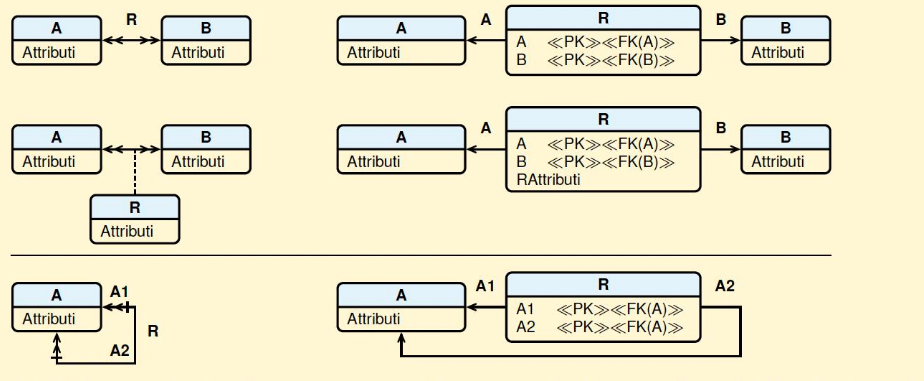
\includegraphics[scale=0.45]{trasfmoltimolti.png}
\end{center}

\subsubsection{Gerarchie tra classi}
Il modello relazionale non può rappresentare le gerarchia tra classi. Bisogna quindi eliminarle e sostituirle con classi e relazioni usando le seguenti tecniche:
\begin{itemize}
	\item \textbf{Relazione unica}: accorpamento delle figlie nel genitore
	\item \textbf{Partizionamento orizzontale}: accorpamento del genitore nelle figlie
	\item \textbf{Partizionamento verticale}: sostituzione della gerarchia con relazioni
\end{itemize}

\paragraph{Relazione unica}
Si seguono i seguenti passi:
\begin{enumerate}
	\item Se $A_0$ è la classe genitore di $A_1$ ed $A_2$, queste ultime vengono eliminate ed accorpate alla prima
	\item Ad $A_0$ viene aggiunto un attributo (\textbf{discriminatore}) che indica da quale delle classi figlie deriva una certa istanza, e gli attributi di $A_1$ ed $A_2$ vengono assorbiti dalla classe genitore, e assumono valore nullo sulle istanze provenienti dall’altra classe
	\item Infine, una relazione relativa a solo una delle classi figlie viene acquisita dalla classe genitore e avrà comunque cardinalità minima uguale a $0$, in quanto gli elementi dell’altra classe non contribuiscono alla relazione.
\end{enumerate}

\begin{center}
	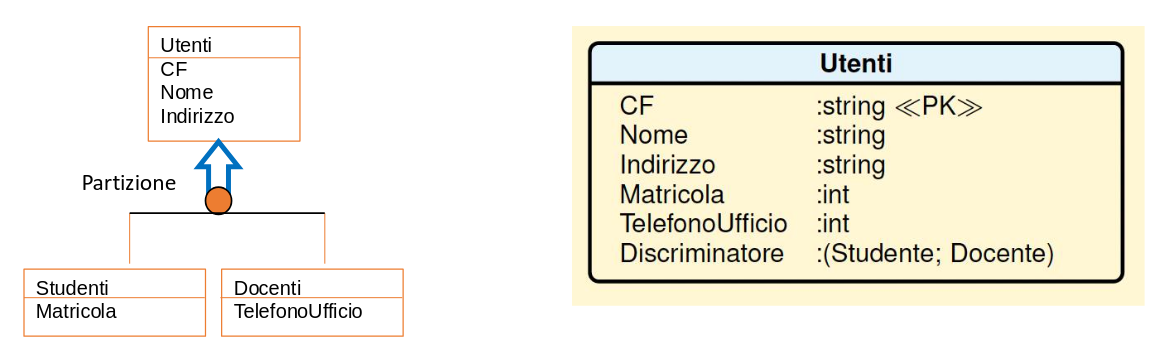
\includegraphics[scale=0.35]{relunica.png}
\end{center}

\newpage
\paragraph{Partizionamento orizzontale}
Se $A_0$ è la classe genitore di $A_1$ ed $A_2$, la classe genitore viene eliminata, e le classi figlie ereditano le proprietà (attributi,identificatore e relazioni) della classe genitore.

\begin{center}
	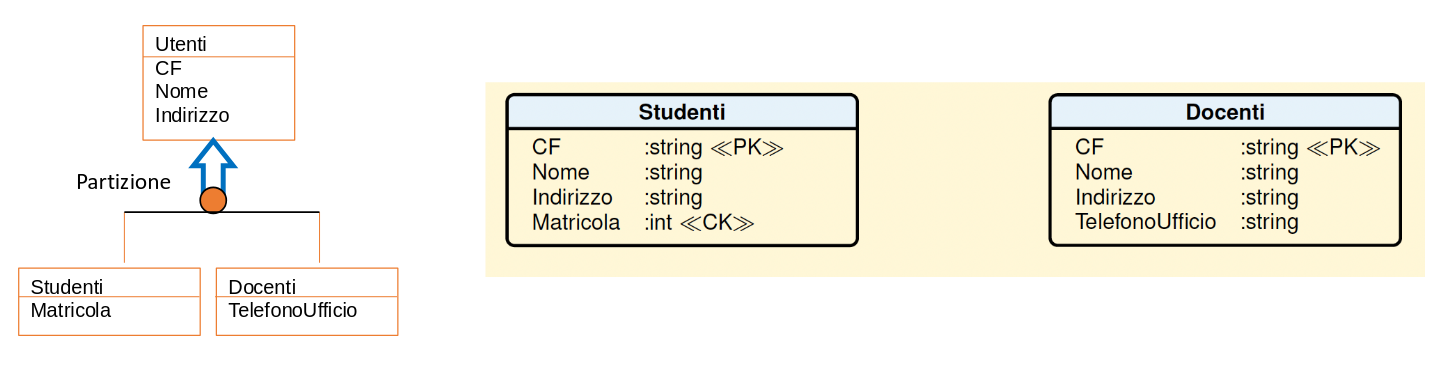
\includegraphics[scale=0.3]{partorizz.png}
\end{center}

\begin{note}
	Questa tecnica divide gli elementi della superclasse $A_0$ in più relazioni diverse, per cui non è possibile mantenere un vincolo referenziale verso $A_0$. In conclusione, questa tecnica non si usa se
	nello schema relazionale c’è una associazione diretta verso $A_0$, ovvero che entra nella superclasse.
\end{note}

\paragraph{Partizionamento verticale}
In questo caso non c’è un trasferimento di attributi o di associazioni e le classi figlie $A_1$ ed $A_2$ sono identificate esternamente dalla classe genitore $A_0$. Nello schema ottenuto vanno aggiunti dei vincoli: ogni occorrenza di $A_0$ non può partecipare contemporaneamente alle due associazioni, e se la gerarchia è totale, deve partecipare ad almeno una delle due.

\begin{center}
	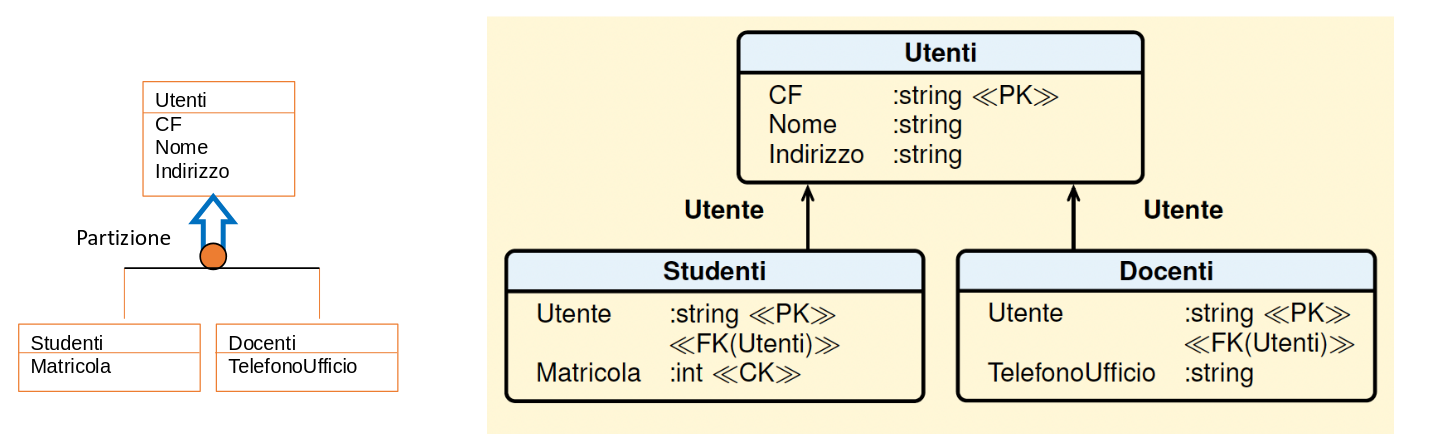
\includegraphics[scale=0.3]{partvert.png}
\end{center}

\subsubsection{Chiavi primarie}
È necessario definire per ogni relazione un insieme di attributi che funga da chiave primaria, seguendo questi passi:
\begin{enumerate}
	\item Si considerano le relazioni che corrispondono a classi dello schema originale	che erano prive di superclassi (\textbf{classi radice}). La chiave primaria è di norma un attributo artificiale, tipicamente un numero progressivo	assegnato dal sistema. E’ possibile utilizzare un attributo presente nella classe, purché
	l’attributo sia \textbf{univoco}, \textbf{totale} e \textbf{costante}.
	\item Per ogni relazione dello schema che corrisponde ad una \textbf{sottoclasse} dello schema originario, la chiave primaria sarà la stessa della superclasse.
	\item Per le relazioni che corrispondono ad $\mathbf{N:M}$ nello schema originario, la chiave primaria sarà costituita dalla concatenazione delle chiavi esterne.
\end{enumerate}

\newpage
\subsubsection{Attributi multivalore}
Una proprietà multivalore di una classe $C$ si rappresenta eliminando il corrispondente attributo da $C$ e creando una nuova relazione $N$ con una chiave di due attributi:
\begin{itemize}
	\item una \textbf{chiave esterna} che fa riferimento alla chiave primaria di $C$
	\item un \textbf{attributo} che corrisponde all’attributo multivalore da trasformare
\end{itemize}
Un oggetto di $C$ con chiave primaria $k$ ed in cui l’attributo assume valore $a_1, \ldots, a_n$ si rappresenta poi inserendo nella relazione $N$ le coppie $(k, a_1), \ldots , (k, a_n)$

\begin{center}
	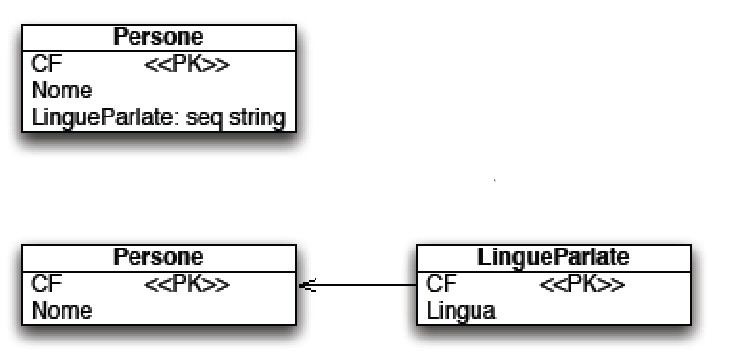
\includegraphics[scale=0.4]{multival.png}
\end{center}

\subsubsection{Attributi composti}
Se un attributo $A_i$ di uno schema di relazione è di tipo $[A_{i1} : T_{i1}, \ldots , A_{ij} :
T_{ij}]$, si sostituisce con gli attributi $A_{i1} : T_{i1}, \ldots, A_{ij} : T_{ij}$. Se $A_i$ faceva parte della chiave primaria dello schema di relazione, si sostituisce $A_i$ con gli attributi $A_{i1}, \ldots, A_{ij}$ nella chiave, e poi si verifica che non esista un sottoinsieme degli attributi della nuova chiave primaria che è esso stesso una chiave.

\begin{example}
	Dato l'attributo composto
	\begin{equation*}
		[\text{Via} : \text{string}, \text{Numero} : \text{int}, \text{Citta}:\text{string}]
	\end{equation*}
	otteniamo
	\begin{center}
		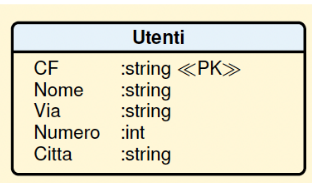
\includegraphics[scale=0.4]{composti.png}
	\end{center}
\end{example}